% Pairing heap represented as a multiway tree.
% Editable source for this diagram. From this directory, regenerate with:
% latex -interaction=nonstopmode -halt-on-error pairing-heap-1.tex
% dvisvgm --no-fonts --exact --bbox=papersize --output=pairing-heap-1.svg pairing-heap-1.dvi
\documentclass[tikz,border=2pt]{standalone}
\usepackage{lmodern}
\usepackage{tikz}
\usetikzlibrary{arrows.meta,backgrounds,shapes.geometric,patterns}
\definecolor{linkred}{HTML}{B5240A}
\definecolor{noteBlue}{HTML}{0067A5}
\definecolor{softgreen}{HTML}{D8EAD0}
\definecolor{softpurple}{HTML}{D9D1E8}
\definecolor{softpink}{HTML}{F5CECF}
\definecolor{softyellow}{HTML}{FFF2C9}
\begin{document}
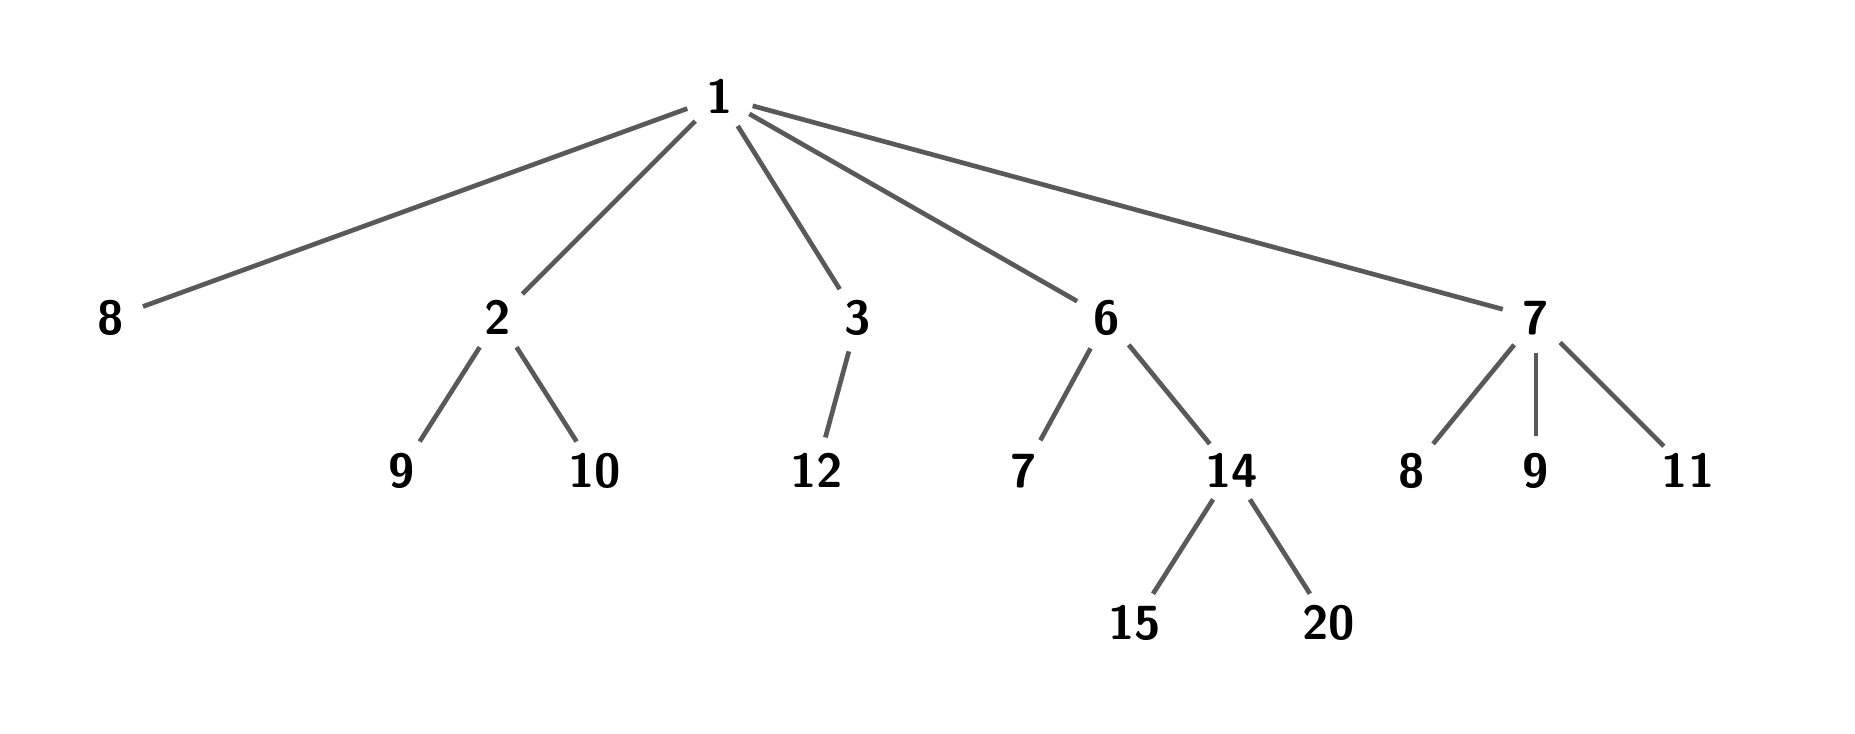
\begin{tikzpicture}[x=1pt,y=-1pt,>=Stealth,line cap=round,line join=round]
\path[use as bounding box] (0,0) rectangle (650,245);
\begin{scope}[on background layer]

\end{scope}
\node[circle,draw=none,fill=white,text=black,minimum size=24pt,inner sep=0pt,line width=0.8pt,font=\sffamily\fontsize{17}{20.4}\selectfont,font=\sffamily\bfseries\fontsize{17}{20}\selectfont] (r) at (250,25) {1};
\node[circle,draw=none,fill=white,text=black,minimum size=24pt,inner sep=0pt,line width=0.8pt,font=\sffamily\fontsize{17}{20.4}\selectfont,font=\sffamily\bfseries\fontsize{17}{20}\selectfont] (a) at (30,105) {8};
\node[circle,draw=none,fill=white,text=black,minimum size=24pt,inner sep=0pt,line width=0.8pt,font=\sffamily\fontsize{17}{20.4}\selectfont,font=\sffamily\bfseries\fontsize{17}{20}\selectfont] (b) at (170,105) {2};
\node[circle,draw=none,fill=white,text=black,minimum size=24pt,inner sep=0pt,line width=0.8pt,font=\sffamily\fontsize{17}{20.4}\selectfont,font=\sffamily\bfseries\fontsize{17}{20}\selectfont] (c) at (300,105) {3};
\node[circle,draw=none,fill=white,text=black,minimum size=24pt,inner sep=0pt,line width=0.8pt,font=\sffamily\fontsize{17}{20.4}\selectfont,font=\sffamily\bfseries\fontsize{17}{20}\selectfont] (d) at (390,105) {6};
\node[circle,draw=none,fill=white,text=black,minimum size=24pt,inner sep=0pt,line width=0.8pt,font=\sffamily\fontsize{17}{20.4}\selectfont,font=\sffamily\bfseries\fontsize{17}{20}\selectfont] (e) at (545,105) {7};
\node[circle,draw=none,fill=white,text=black,minimum size=24pt,inner sep=0pt,line width=0.8pt,font=\sffamily\fontsize{17}{20.4}\selectfont,font=\sffamily\bfseries\fontsize{17}{20}\selectfont] (b1) at (135,160) {9};
\node[circle,draw=none,fill=white,text=black,minimum size=24pt,inner sep=0pt,line width=0.8pt,font=\sffamily\fontsize{17}{20.4}\selectfont,font=\sffamily\bfseries\fontsize{17}{20}\selectfont] (b2) at (205,160) {10};
\node[circle,draw=none,fill=white,text=black,minimum size=24pt,inner sep=0pt,line width=0.8pt,font=\sffamily\fontsize{17}{20.4}\selectfont,font=\sffamily\bfseries\fontsize{17}{20}\selectfont] (c1) at (285,160) {12};
\node[circle,draw=none,fill=white,text=black,minimum size=24pt,inner sep=0pt,line width=0.8pt,font=\sffamily\fontsize{17}{20.4}\selectfont,font=\sffamily\bfseries\fontsize{17}{20}\selectfont] (d1) at (360,160) {7};
\node[circle,draw=none,fill=white,text=black,minimum size=24pt,inner sep=0pt,line width=0.8pt,font=\sffamily\fontsize{17}{20.4}\selectfont,font=\sffamily\bfseries\fontsize{17}{20}\selectfont] (d2) at (435,160) {14};
\node[circle,draw=none,fill=white,text=black,minimum size=24pt,inner sep=0pt,line width=0.8pt,font=\sffamily\fontsize{17}{20.4}\selectfont,font=\sffamily\bfseries\fontsize{17}{20}\selectfont] (d21) at (400,215) {15};
\node[circle,draw=none,fill=white,text=black,minimum size=24pt,inner sep=0pt,line width=0.8pt,font=\sffamily\fontsize{17}{20.4}\selectfont,font=\sffamily\bfseries\fontsize{17}{20}\selectfont] (d22) at (470,215) {20};
\node[circle,draw=none,fill=white,text=black,minimum size=24pt,inner sep=0pt,line width=0.8pt,font=\sffamily\fontsize{17}{20.4}\selectfont,font=\sffamily\bfseries\fontsize{17}{20}\selectfont] (e1) at (500,160) {8};
\node[circle,draw=none,fill=white,text=black,minimum size=24pt,inner sep=0pt,line width=0.8pt,font=\sffamily\fontsize{17}{20.4}\selectfont,font=\sffamily\bfseries\fontsize{17}{20}\selectfont] (e2) at (545,160) {9};
\node[circle,draw=none,fill=white,text=black,minimum size=24pt,inner sep=0pt,line width=0.8pt,font=\sffamily\fontsize{17}{20.4}\selectfont,font=\sffamily\bfseries\fontsize{17}{20}\selectfont] (e3) at (600,160) {11};
\begin{scope}[on background layer]
\draw[draw=black!65,line width=1.7pt] (r) -- (a);
\draw[draw=black!65,line width=1.7pt] (r) -- (b);
\draw[draw=black!65,line width=1.7pt] (r) -- (c);
\draw[draw=black!65,line width=1.7pt] (r) -- (d);
\draw[draw=black!65,line width=1.7pt] (r) -- (e);
\draw[draw=black!65,line width=1.7pt] (b) -- (b1);
\draw[draw=black!65,line width=1.7pt] (b) -- (b2);
\draw[draw=black!65,line width=1.7pt] (c) -- (c1);
\draw[draw=black!65,line width=1.7pt] (d) -- (d1);
\draw[draw=black!65,line width=1.7pt] (d) -- (d2);
\draw[draw=black!65,line width=1.7pt] (d2) -- (d21);
\draw[draw=black!65,line width=1.7pt] (d2) -- (d22);
\draw[draw=black!65,line width=1.7pt] (e) -- (e1);
\draw[draw=black!65,line width=1.7pt] (e) -- (e2);
\draw[draw=black!65,line width=1.7pt] (e) -- (e3);
\end{scope}

\end{tikzpicture}
\end{document}
